\documentclass[main.tex]{subfiles}
\begin{comment}
\usepackage{geometry}   
\usepackage{graphicx}
\usepackage{amssymb}
\usepackage{amsmath}
\usepackage{mathtools}% http://ctan.org/pkg/mathtools
\usepackage{float}
\newcommand\tab[1][1cm]{\hspace*{#1}}
\geometry{letterpaper}  
\usepackage{tabu}
\usepackage{verbatim}
\usepackage [english]{babel}
\MakeOuterQuote{"}
\usepackage{multicol}
\setlength{\columnsep}{1cm}
\end{comment}
\begin{document}
%\begin{multicols}{2}[]
\normalsize

\begin{center}\section{Experiments}\end{center}
As mentioned before, the provided equation calculates the maximum number of rounds needed to receive a file. To mimic this situation in the experiments, we randomly changed the position of the corrupted channels after every round. \paragraph{}To test the efficiency of these protocols, we implemented them simulating a real word scenario. Note that we implemented the protocols using normal TCP channels since it doesn't make any difference if they were covert channels or normal channels. Through out the experiments we consider our computer running $(macOS  10.13.4)$ positioned in Rome as the victim having these characteristics:
\begin{itemize}
\item CPU: $4$.
\item Processor: Intel Core i$5$.
\item Clock Speed: 2,5 GHz.
\item Memory: $8$GB.
\end{itemize}
While the attacker server is a rented machine running $(ubuntu-xenial-16.04)$ from amazon located in Sydney "Australia" with the characteristics below:
\begin{itemize}
\item vCPU: $1$.
\item Processor: Intel Xeon.
\item Clock Speed: 2,5 GHz.
\item Memory: $1$GB.
\end{itemize}
To check how the number of corrupted channels with respect to the number of total available channels affects the efficiency and the number of rounds it takes the protocol to send a file. We conducted the following experiments with a file of size $6MB$ that will be divided into $93$ packets:\paragraph{}
We repeated the same experiments with a larger file $40MB$ that is divided into $230$ packets in total.\\
The graphs below will show how the total number of rounds required to send the file change when increasing the number of corrupted channels using protocol $\#2$ and the equation (Fig. $\#23)$. In addition in (Fig. $\#24)$ we compared them with protocol $\#1$. By using a total $10$ channels.\\

\begin{figure} [!htb]\centering
  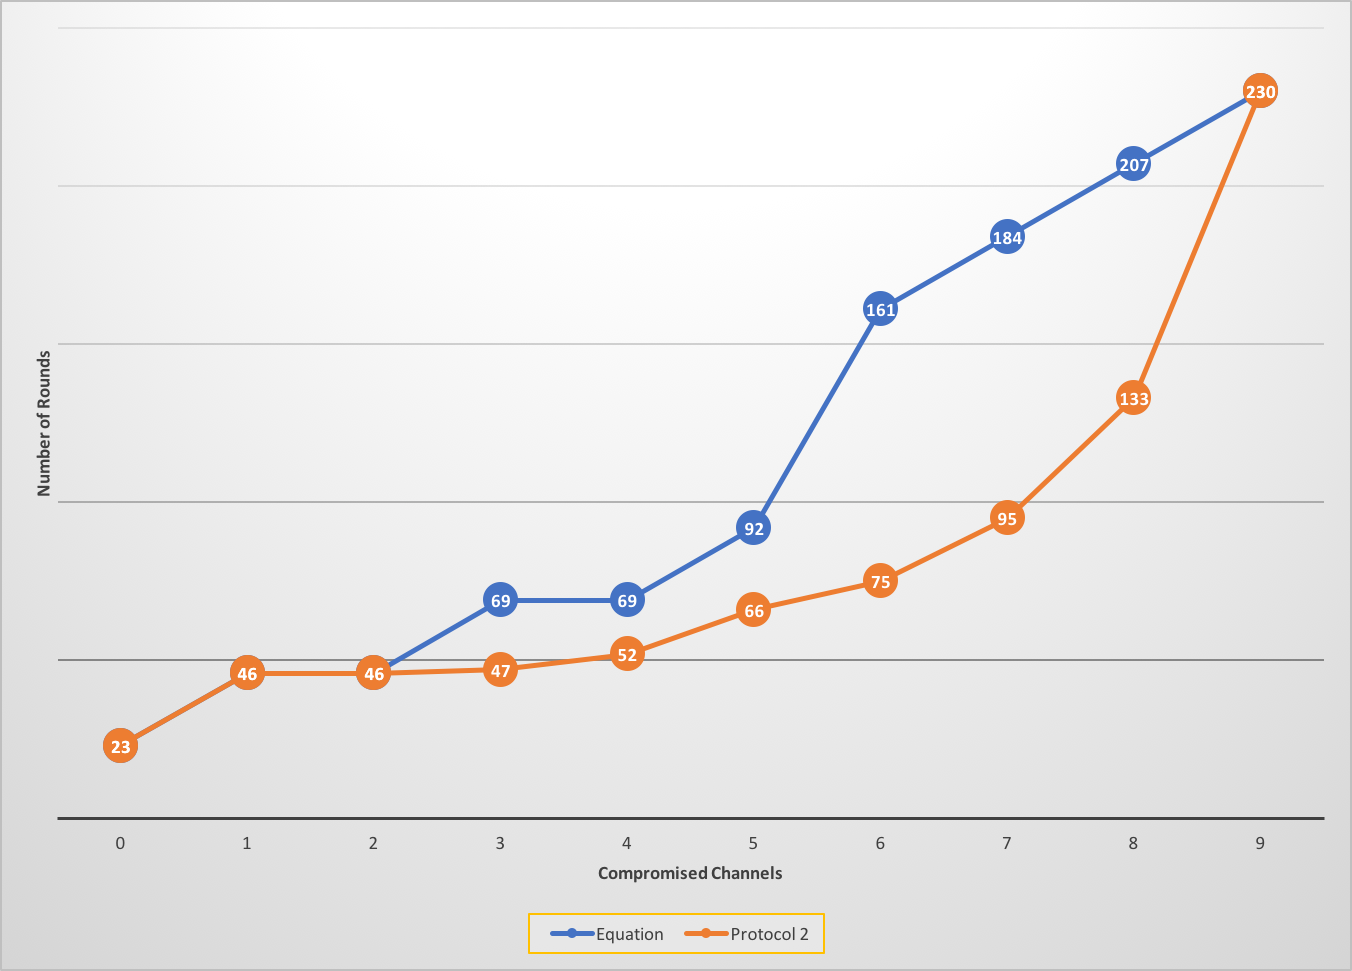
\includegraphics[keepaspectratio, width=8cm]{pics/10Pro2Eq.png}
 \caption{The difference in number of rounds taken protocol $\#2$, and the equation}%\end{figure}\clearpage

%\begin{figure} [!htb]\centering
 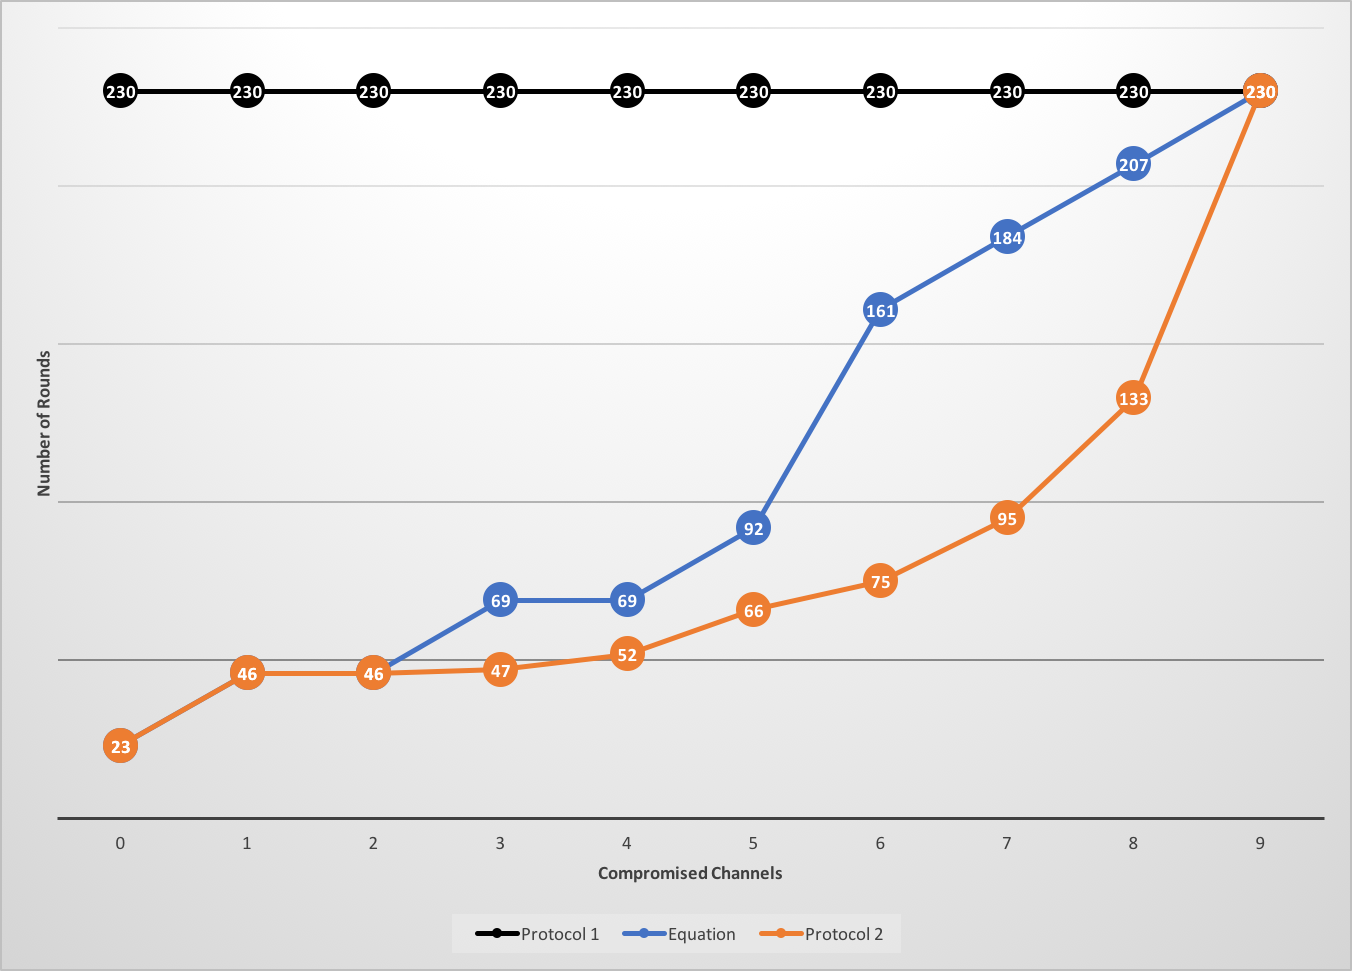
\includegraphics[keepaspectratio, width=8cm]{pics/10Complete.png}
 \caption{The difference in number of rounds taken protocol $\#2$, $\#1$ and the equation}\end{figure}
 
 The graphs below will show how the total number of rounds required to send the file changes when increasing the number of corrupted channels using protocol $\#2$ and the equation (Fig. $\#25)$. In addition in (Fig. $\#26)$ we compared them with protocol $\#1$. By using a total of $20$ channels.\\
\begin{figure}[!htb]
\centering
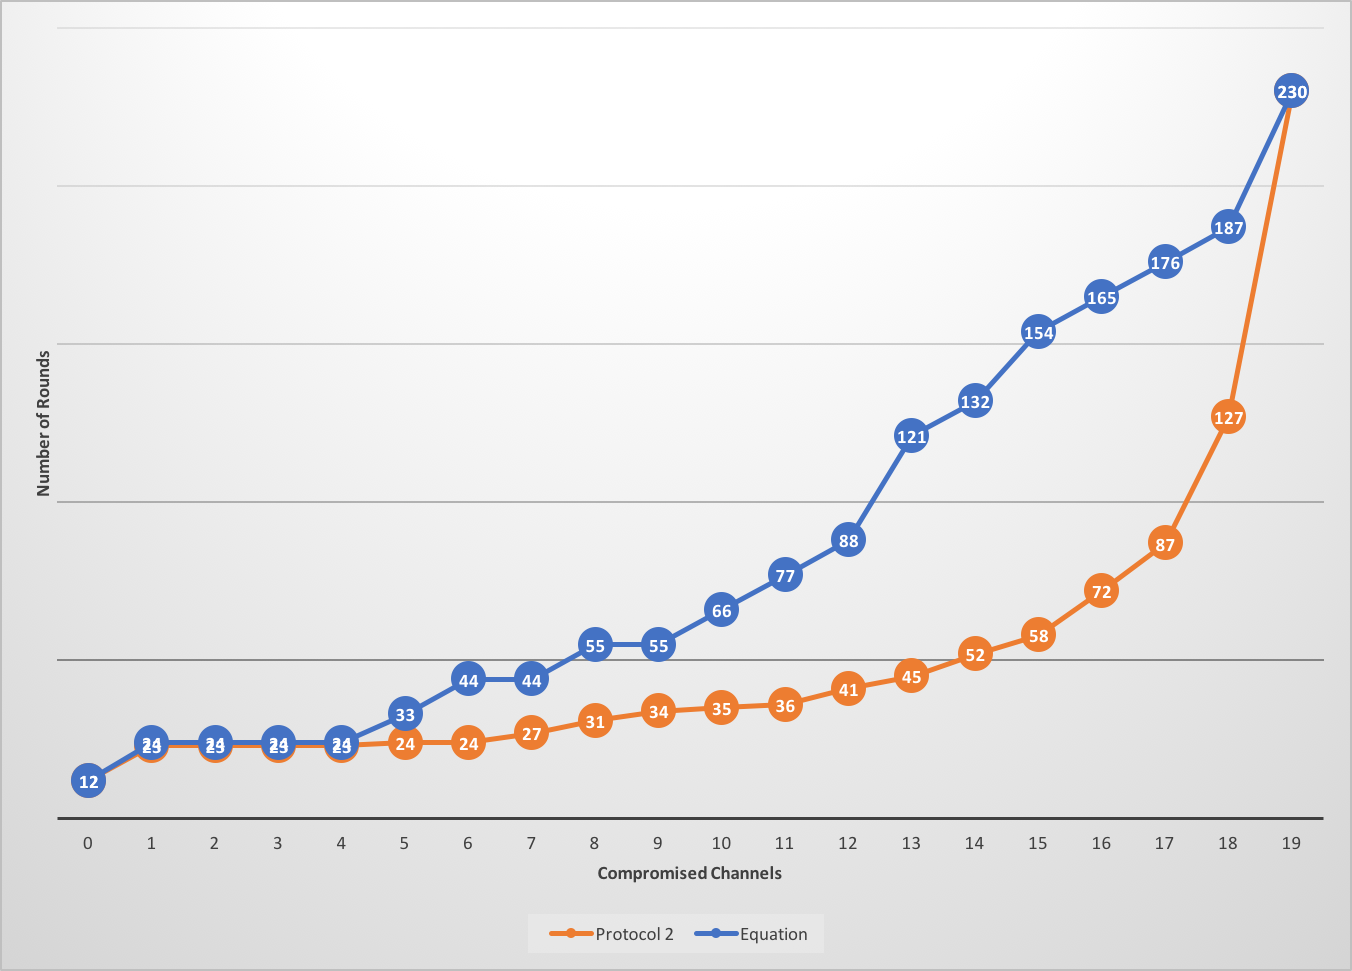
\includegraphics[keepaspectratio, width=8cm]{pics/20Pro2Eq.png}
\caption{The difference in number of rounds taken protocol $\#2$, and the equation}
\end{figure}
\begin{figure}[!htb]
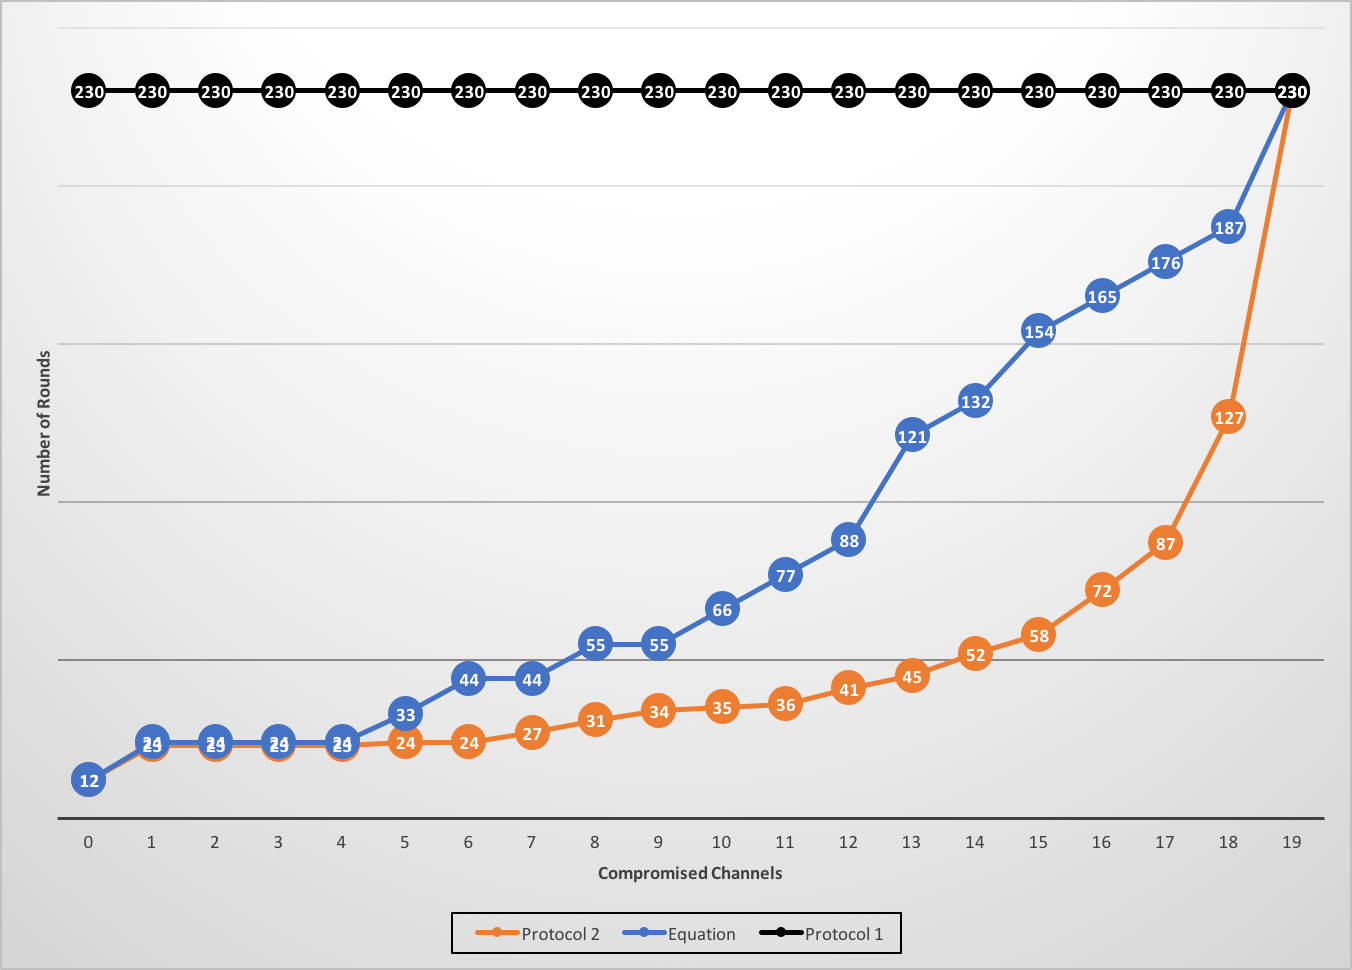
\includegraphics[keepaspectratio, width=8cm]{pics/20Complete.png}
\caption{The difference in number of rounds taken protocol $\#2$, $\#1$ and the equation}
\end{figure}

The graphs below will show how the total number of rounds required to send the file changes when increasing the number of corrupted channels using protocol $\#2$ and the equation (Fig. $\#27)$. In addition in (Fig. $\#28)$ we compared them with protocol $\#1$. By using a total of $30$ channels.
\begin{figure} [!htb]\centering
 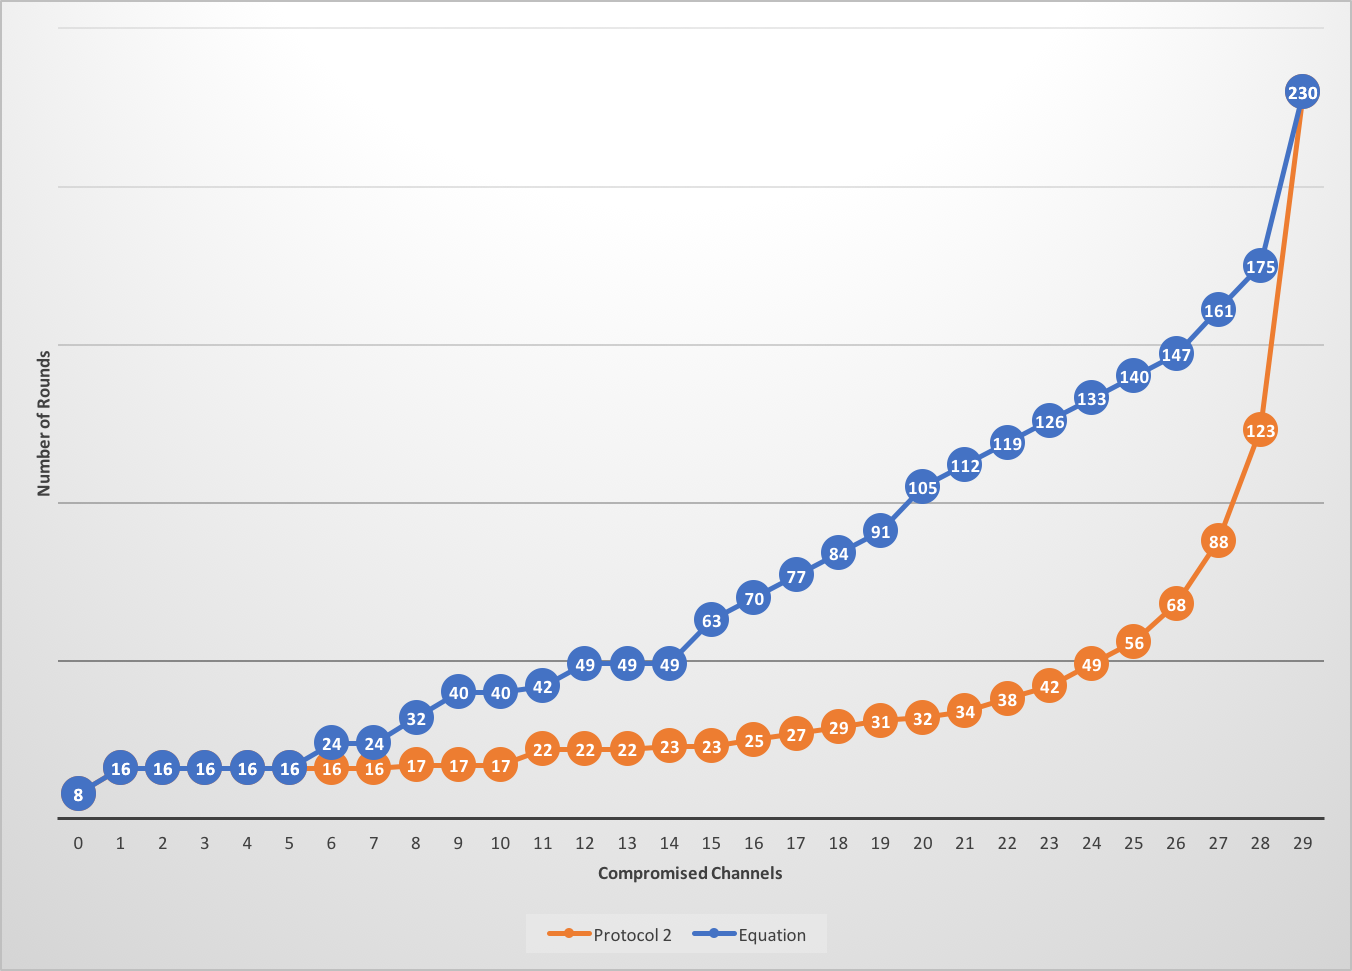
\includegraphics[keepaspectratio, width=8cm]{pics/30Pro2Eq.png}
 \caption{The difference in number of rounds taken protocol $\#2$ and the equation}%\end{figure}
 %\clearpage
% \begin{figure} [!htb]\centering
 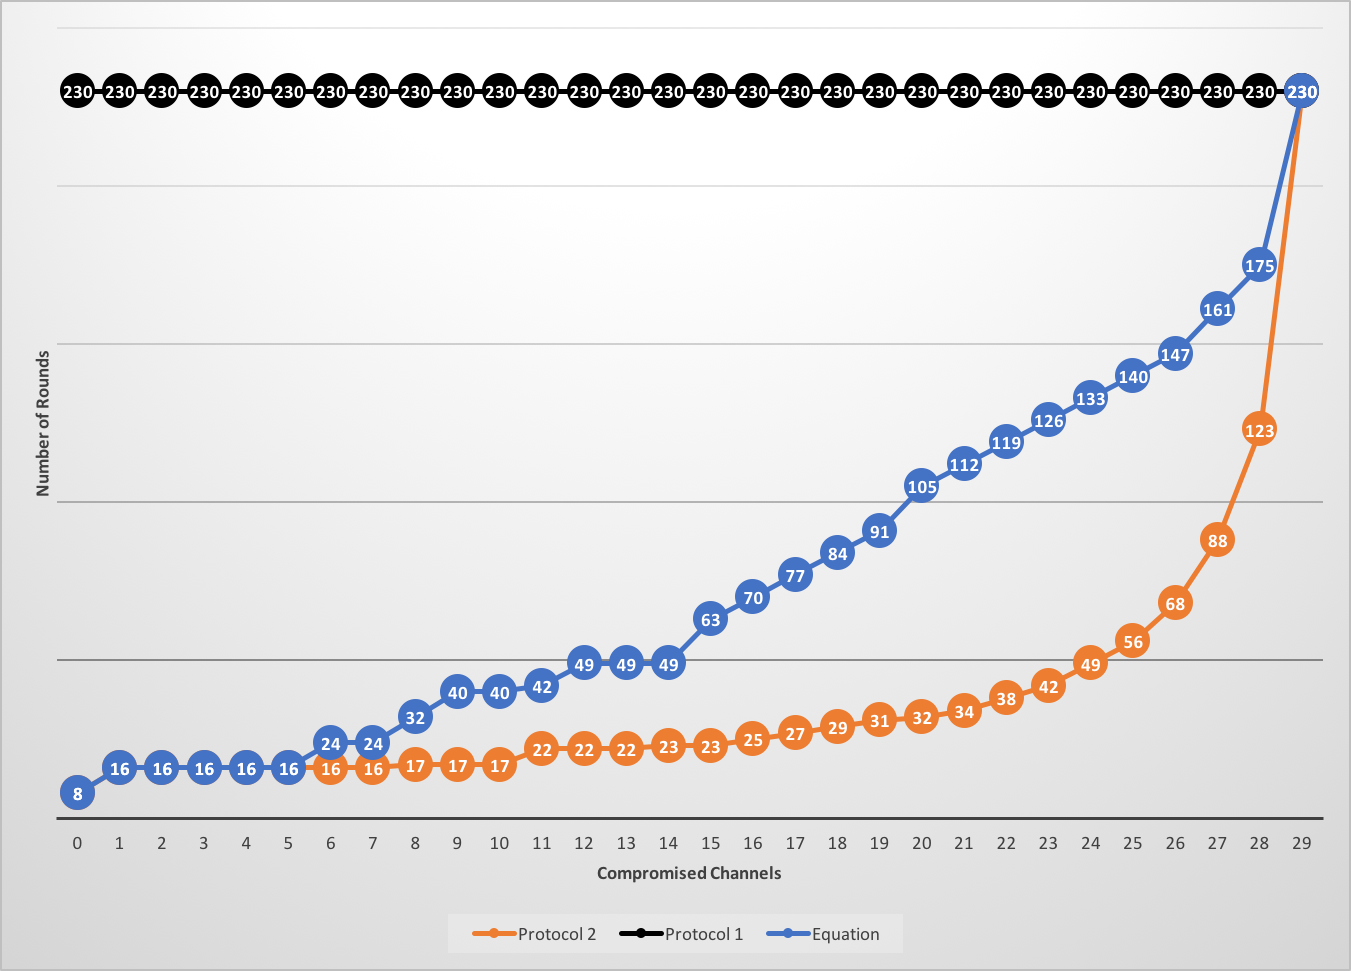
\includegraphics[keepaspectratio, width=8cm]{pics/30Complete.png}
 \caption{The difference in number of rounds taken protocol $\#2$, $\#1$ and the equation}\end{figure}
 
 The graphs below will show how the efficiency of the protocols is changing with respect to the number of corrupted channels.\begin{itemize}
 \item With a total number of 10 channels. (Fig. $\#29)$. 
  \item With a total number of 20 channels. (Fig. $\#30)$.
   \item With a total number of 30 channels. (Fig. $\#31)$.\end{itemize}\begin{figure} [!htb]\centering
 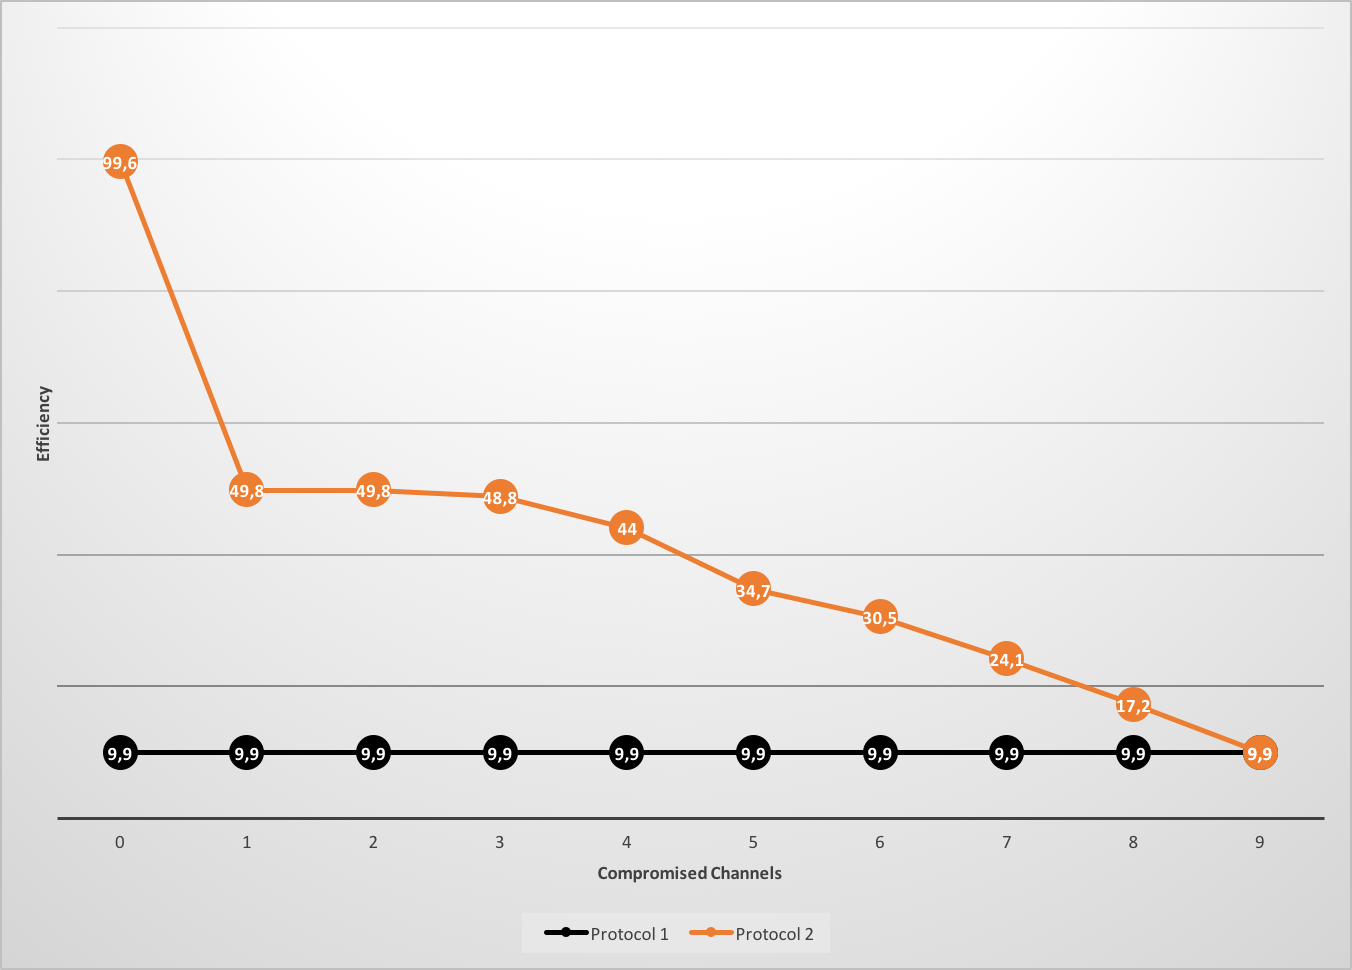
\includegraphics[keepaspectratio, width=8cm]{pics/10Eff.png}
 \caption{The efficiency of protocols $\#1$ \& $\#2$ w.r.t the compromised channels.}\end{figure}
\begin{figure} [!htb]\centering 
\centering
 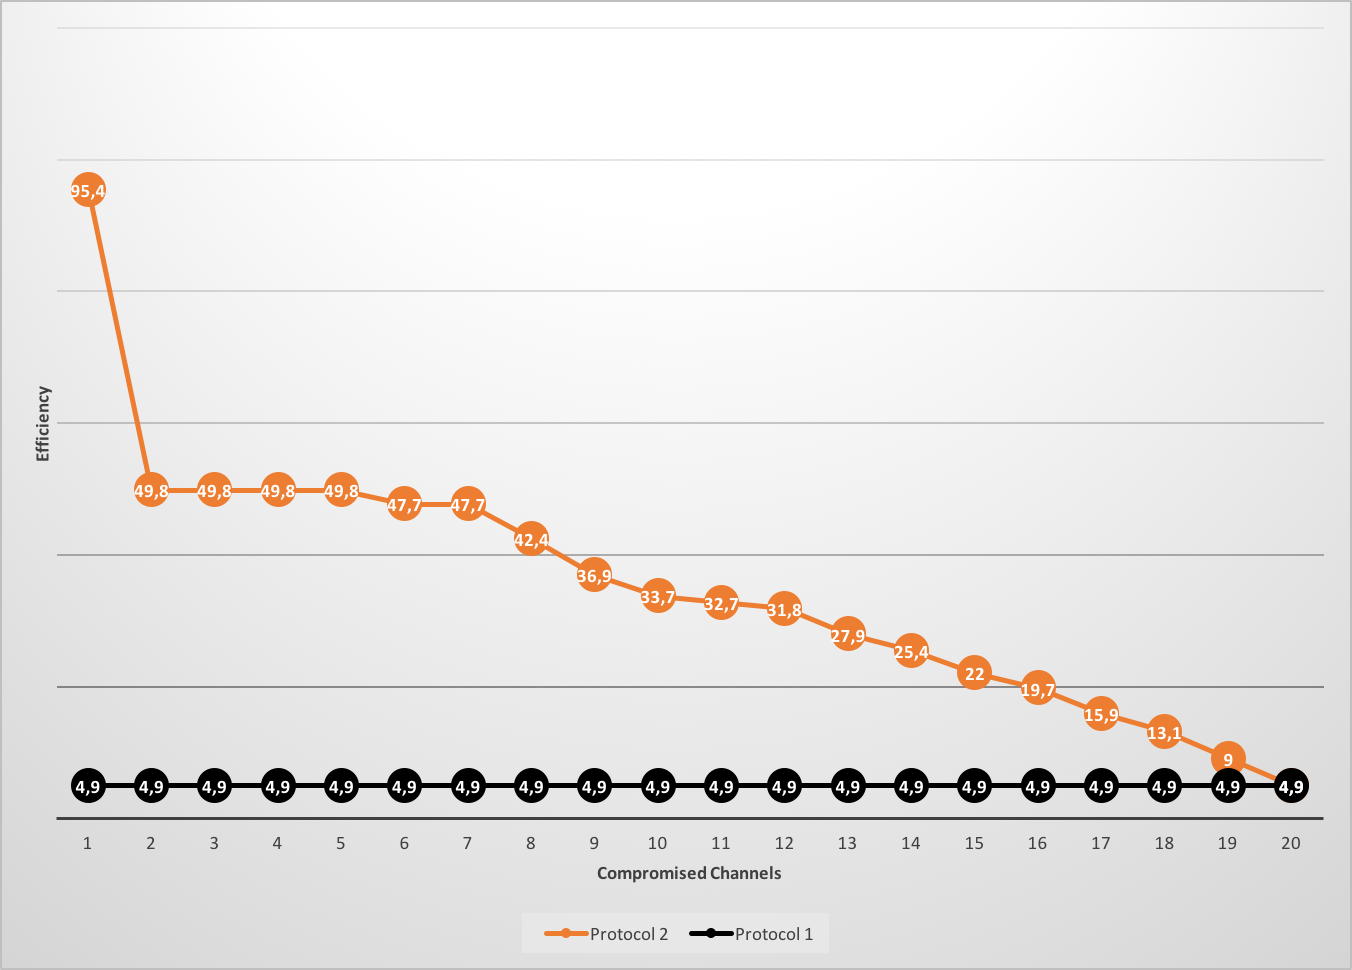
\includegraphics[keepaspectratio, width=8cm]{pics/20Eff.png}
 \caption{The efficiency of protocols $\#1$ \& $\#2$ w.r.t the compromised channels.}%\end{figure}
 %\clearpage
 %\begin{figure}
\centering
 \includegraphics[keepaspectratio, width=8cm]{pics/30eff.png}
 \caption{The efficiency of protocols $\#1$ \& $\#2$ w.r.t the compromised channels.}\end{figure}

\subsection{Analysis}
\subsubsection{General Notes:}
\paragraph{}As before, we notice that Protocol $\#1$ always needs a fixed number of rounds to send the file regardless of the number of available channels or the number of corrupted channels. And the number of rounds is the same as the number of packets to be sent which is expected from protocol $\#1$ as it broadcasts every packet over all the channels at each round. So, by having for example, $10$ packets the protocol will broadcast $1$ packet in every round and therefore, to send $10$ packets, it will take $10$ rounds.
\paragraph{}Now, by moving to protocol $\#2$ we can notice that, with $0$ compromised channels, when we increase the number of total available channels, the number of rounds needed to send the file decreases.
\paragraph{}With only $1$ channel that is not compromised, we can notice that protocol $\#2$ acts in the same way as protocol  $\#1$, since at every round only $1$ packet is correctly received.  
\subsubsection{Case Study: Figure $\#23$}
\begin{itemize}
\item \textbf{\textit{X-axis}}: Shows the number of compromised/bad channels.
\item \textbf{\textit{Y-axis}}: Shows the number of rounds taken to completely send the file.
\item \textbf{\textit{Blue line}}: The number of rounds calculated by the equation.
\item \textbf{\textit{Orange line}}: The number of rounds extracted from the experiments.
\end{itemize}
This graph visualises how many rounds have taken the equation and the experiments to send the file over the number of compromised channels.
\paragraph{Analyzing points}
\begin{itemize}
\item \textbf{\textit{$0$ Compromised Channels}}: Both the protocol and the equation takes the lowest number of rounds possible to send the file.
\item \textbf{\textit{$3$ Compromised Channels}}: A turning point for both the equation line and the experiments.
\item \textbf{\textit{$9$ Compromised Channels}}: The peak of both the equation and the experiments lines.
\end{itemize}
\paragraph{comparing trends:}
\begin{itemize}
\item \textbf{\textit{$0-2$ Compromised Channels}}: The lines of both the protocol and the equation slightly increase but still taking the same number of rounds to send the file.
\item \textbf{\textit{$3-8$ Compromised Channels}}: The lines of both the equation and the experiment increase where the line of the experiment is always higher.
\item \textbf{\textit{$8-9$ Compromised Channels}}: The line of the equation slightly increases till it reaches its maximum point while the line of the experiments increases rapidly to reach its maximum point.
\end{itemize}

\subsubsection{Case Study: Figure $\#25$}
\begin{itemize}
\item \textbf{\textit{X-axis}}: Shows the number of compromised/bad channels.
\item \textbf{\textit{Y-axis}}: Shows the number of rounds taken to completely send the file.
\item \textbf{\textit{Blue line}}: The number of rounds calculated by the equation.
\item \textbf{\textit{Orange line}}: The number of rounds extracted from the experiments of protocol $\#2$.
\end{itemize}
This graph visualises how many rounds taken the equation, and the experiments of protocol $\#2$ to send the file with respect to the number of compromised channels.
\paragraph{Analyzing points}
\begin{itemize}
\item \textbf{\textit{$0$ Compromised Channels}}: Both the protocol and the equation takes the lowest number of rounds possible to send the file.
\item \textbf{\textit{$3$ Compromised Channels}}: A turning point for the equation line.
\item \textbf{\textit{$7$ Compromised Channels}}: A turning point for the experiments line.
\item \textbf{\textit{$12$ Compromised Channels}}: The turning of the equation line where it started to increase significantly.
\item \textbf{\textit{$17$ Compromised Channels}}: The turning of the experiments line where it started to increase rapidly.  
\item \textbf{\textit{$19$ Compromised Channels}}: The peak of both the equation and the experiments lines.  
\end{itemize}
\paragraph{comparing trends:}
\begin{itemize}
\item \textbf{\textit{$0-4$ Compromised Channels}}: Both the protocol and the equation slightly increases but still taking the same number of rounds to send the file.
\item \textbf{\textit{$5-12$ Compromised Channels}}: The equation line is steadily increasing.
\item \textbf{\textit{$7-17$ Compromised Channels}}: The experiment line is steadily increasing.
\item \textbf{\textit{$12-19$ Compromised Channels}}: The equation line is rapidly increasing till it reaches its maximum point.
\item \textbf{\textit{$17-19$ Compromised Channels}}: The experiment line is rapidly increasing till it reaches its maximum point.
\end{itemize}

\subsubsection{Case Study: Figure $\#27$}
\begin{itemize}
\item \textbf{\textit{X-axis}}: Shows the number of compromised/bad channels.
\item \textbf{\textit{Y-axis}}: Shows the number of rounds taken to completely send the file.
\item \textbf{\textit{Blue line}}: The number of rounds calculated by the equation.
\item \textbf{\textit{Orange line}}: The number of rounds extracted from the experiments.
\end{itemize}
This graph visualises how many rounds taken the equation, and the experiments of protocol $\#2$ to send the file over the number of compromised channels.
\paragraph{Analyzing points}
\begin{itemize}
\item \textbf{\textit{$0$ Compromised Channels}}: Both the protocol and the equation takes the lowest number of rounds possible to send the file.
\item \textbf{\textit{$5$ Compromised Channels}}: A turning point for the equation line.
\item \textbf{\textit{$27$ Compromised Channels}}: The turning of the experiments line where it started to increase rapidly.  
\item \textbf{\textit{$29$ Compromised Channels}}: The peak of both the equation and the experiments lines.  
\end{itemize}
\paragraph{comparing trends:}
\begin{itemize}
\item \textbf{\textit{$0-5$ Compromised Channels}}: Both the lines of the protocol and the equation slightly increase but still taking the same number of rounds to send the file.
\item \textbf{\textit{$5-28$ Compromised Channels}}: The equation line is steadily increasing.
\item \textbf{\textit{$11-28$ Compromised Channels}}: The experiment line is increasing little by little.
\item \textbf{\textit{$28-29$ Compromised Channels}}: The equation line is rapidly increasing till it reaches its maximum point.
\item \textbf{\textit{$28-29$ Compromised Channels}}: The experiment line is rapidly increasing till it reaches its maximum point.
\end{itemize}
\paragraph{}
Now, we can confirm the proportional relation between the number of corrupted channels and the number of rounds it takes the protocol to send a file. In other words, as the number of corrupted channels increases, the number of rounds will also increases.\\
\subsubsection{Case Study: Figures ($\#29, \#30 \& \#31$)}
\begin{itemize}
\item \textbf{\textit{X-axis}}: Shows the number of compromised/bad channels.
\item \textbf{\textit{Y-axis}}: Shows the efficiency of each protocol.
\item \textbf{\textit{Black line}}: The efficiency of protocol $\#1$.
\item \textbf{\textit{Orange line}}: The efficiency of protocol $\#2$.\end{itemize}
These graphs visualise the efficiency of protocols $\#1$ and $\#2$ with respect to the number of compromised channels.
\paragraph{}
By looking at the three figures, as we noticed from the first experiment the line of protocol $\#1$ is always steady in each figure, and the efficiency is decreasing by increasing the number of total channels. Moreover, the efficiency and the number of compromised channels are independent. And that is because protocol $\#1$ is broadcasting the same packet over all the channels at each round. Plus,  by increasing the number of channels, we're sending more packets. And with that we're making it less efficient. Therefore, we can say that, the efficiency protocol $\#1$ is inversely proportional to the total number of available channels.
\paragraph{Analyzing trends of protocol $\#2$}

\begin{enumerate}
\item \textbf{\textit{For Figure $\#29$}}:
\begin{itemize}
\item \textbf{\textit{$0 - 1$ Compromised Channels}}: The efficiency is at its maximum but it starts decreasing quickly.\item \textbf{\textit{$1 - 2$ Compromised Channels}}: The efficiency is stable.
\item \textbf{\textit{$2 - 9$ Compromised Channels}}: The efficiency is decreasing steadily till it reaches its minimum point.
\end{itemize}
\item \textbf{\textit{For Figure $\#30$}}:
\begin{itemize}
\item \textbf{\textit{$0 - 1$ Compromised Channels}}: The efficiency is at its maximum but it starts decreasing quickly.\item \textbf{\textit{$1 - 5$ Compromised Channels}}: The efficiency is stable.
\item \textbf{\textit{$5 - 19$ Compromised Channels}}: The efficiency is decreasing steadily till it reaches its minimum point.
\end{itemize}
\item \textbf{\textit{For Figure $\#31$}}:
\begin{itemize}
\item \textbf{\textit{$0 - 1$ Compromised Channels}}: The efficiency is at its maximum but it starts decreasing quickly.\item \textbf{\textit{$1 - 7$ Compromised Channels}}: The efficiency is stable.
\item \textbf{\textit{$7 - 10$ Compromised Channels}}: The efficiency is slightly decreasing.
\item \textbf{\textit{$10 - 11$ Compromised Channels}}: The efficiency is quickly decreasing.
\item \textbf{\textit{$11 - 29$ Compromised Channels}}: The efficiency is decreasing steadily till it reaches its minimum point.
\end{itemize}
\end{enumerate}
\paragraph{}
The same deduction with the first experiment, there is an inverse proportional relation between the number of corrupted channels and the efficiency of protocol $\#2$. In other words, as the number of corrupted channels increases, the efficiency decreases.

\end{document}